%% Listas convertidas em prosa em 15/11/2026: 3 de 3. O enumerate do ciclo do
%% filtro de Kalman foi MANTIDO -- e procedimento sequencial com realimentacao, nao
%% lista "Termo: explicacao".
%% Revisao estilistica em 15/11/2026. Reescritos a abertura (truismo mais
%% metadiscurso "Esta secao apresenta os conceitos essenciais"), o "aspecto
%% crucial" e o paragrafo de fechamento, que repetia o tema com adjetivos
%% elogiosos sem acrescentar conteudo. O fecho agora delimita: nenhuma tecnica
%% de fusao desta secao e implementada na tese, e a secao existe para fixar o
%% que se entende por evento sensorial.
\section{Fusão Sensorial Heterogênea}
\label{sec:fund-fusao}

Nenhuma modalidade sensorial isolada cobre as condições de uma subestação: a câmera perde o alvo sob reflexo metálico, o \ac{LiDAR} não distingue um transformador quente de um frio, o microfone não localiza o que ouve. Esta seção percorre as técnicas que combinam modalidades distintas e os limites de cada uma, para fixar o que este trabalho entende por evento sensorial.

\subsection{Conceitos Fundamentais de Fusão Sensorial}

A fusão sensorial pode ser definida como o processo de integração de dados provenientes de múltiplos sensores, com o objetivo de produzir informações mais precisas, completas e confiáveis do que seria possível utilizando cada sensor individualmente \cite{Hall1997}. Em robótica móvel, a percepção ambiental precisa ser robusta mesmo em condições adversas, como as encontradas em subestações elétricas \cite{Neto2021FiltrosRadarLidar}.

Em sistemas robóticos autônomos, a fusão sensorial busca superar as limitações inerentes a cada tipo de sensor, como limitações de alcance, sensibilidade a condições ambientais, ruído e incerteza nas medições, e interferência eletromagnética - particularmente relevante em subestações elétricas \cite{He2007EMCSubstation}.

A heterogeneidade na fusão sensorial refere-se à integração de dados provenientes de sensores de naturezas fundamentalmente distintas, como sensores visuais (câmeras \ac{RGB}), térmicos (câmeras termográficas), acústicos (microfones), de distância (\ac{LiDAR}, ultrassom), inerciais (\ac{IMU}) e químicos (sensores de gás) \cite{Alatise2020Review}. Esta abordagem multimodal permite uma percepção mais completa do ambiente, explorando as complementaridades entre diferentes modalidades sensoriais.

\subsection{Níveis de Fusão Sensorial}
A fusão sensorial pode ser realizada em diferentes níveis de abstração
\cite{Costa2018ImplementacaoFusao, Santos2023FusaoSensorial}, e o nível escolhido decide
o que se pode recuperar adiante, porque informação descartada no pré-processamento não
volta. Na \emph{fusão Z}, de baixo nível, a combinação ocorre diretamente sobre os sinais
recebidos, como intensidade de luz, distância ou temperatura: é o caso de nuvens de
pontos de múltiplos \ac{LiDAR} combinadas entre si, ou de imagens \ac{RGB} com imagens
térmicas. Na \emph{fusão F}, de nível médio, o que se combina são características já
extraídas por algum pré-processamento, como bordas, objetos detectados e velocidades, de
sorte que a fusão opera sobre vetores de características de imagem e de radar, e não
sobre as amostras brutas. Na \emph{fusão D}, de alto nível, cada sensor processa e
interpreta seus próprios dados antes da combinação, que passa a ser entre decisões: um
sensor classifica ``obstáculo'' e outro ``livre'', e a fusão resolve o conflito pela
confiança atribuída a cada um.

\begin{figure}[h]
    \centering
%% Figura refeita em 14/11/2026. A versao anterior estava errada em dois dos tres
%% niveis: o nivel medio trazia uma caixa DECISAO pendurada no sensor, que nao
%% pertence a esse nivel, e o nivel alto mostrava UM sensor seguido de QUATRO decisoes
%% soltas. As tres faixas tambem tinham estruturas diferentes entre si, de modo que a
%% figura nao deixava ver o unico ponto da taxonomia: onde, no mesmo fluxo, a fusao
%% ocorre. A versao atual usa o mesmo encadeamento nas tres faixas, variando so a
%% posicao da caixa de fusao. Reduzida de \textwidth para 0,85 por ser didatica.
    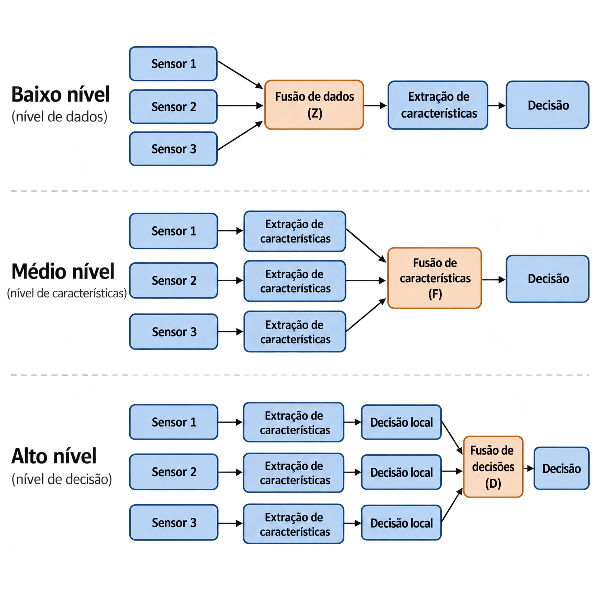
\includegraphics[width=0.85\textwidth]{figuras/fig_niveis_fusao.pdf}
    \caption{Níveis de fusão sensorial: o mesmo encadeamento de três sensores,
    variando o ponto em que a fusão ocorre --- sobre os dados brutos ($Z$), sobre as
    características extraídas ($F$) ou sobre as decisões locais de cada sensor ($D$).}
    \legend{Fonte: Elaborada pelo autor com base em \citeonline{Costa2018ImplementacaoFusao}
    e \citeonline{Santos2023FusaoSensorial}.}
    \label{fig:niveis_fusao}
\end{figure}
A \autoref{fig:niveis_fusao} ilustra os níveis de fusão sensorial.




\subsubsection{Fusão de Baixo Nível (Nível de Dados)}

A fusão de baixo nível envolve a combinação direta dos sinais provenientes dos sensores antes de qualquer extração de características ou interpretação semântica:

\begin{equation}
Z_{fusão} = f(Z_1, Z_2, ..., Z_n)
\end{equation}

Onde $Z_i$ representa os dados brutos do sensor $i$, e $f$ é a função de fusão aplicada.

Exemplos incluem combinação de nuvens de pontos de múltiplos sensores \ac{LiDAR} e fusão de imagens de diferentes espectros (\ac{RGB} + infravermelho). A principal vantagem é a preservação de toda a informação original, mas requer maior capacidade computacional e pode ser sensível a problemas de sincronização temporal e calibração espacial entre sensores \cite{Schneider2018FusaoSensores}.

\subsubsection{Fusão de Médio Nível (Nível de Características)}

A fusão de médio nível opera sobre características extraídas dos dados sensoriais brutos:

\begin{equation}
F_{fusão} = g(F_1, F_2, ..., F_n)
\end{equation}

Onde $F_i$ representa o conjunto de características extraídas do sensor $i$, e $g$ é a função de fusão aplicada às características.

Este nível oferece um bom equilíbrio entre redução de dimensionalidade (e consequentemente de carga computacional) e preservação de informação relevante \cite{Grassi2006ArquiteturaHibrida}.

\subsubsection{Fusão de Alto Nível (Nível de Decisão)}

A fusão de alto nível combina decisões ou classificações já realizadas por algoritmos específicos para cada sensor:

\begin{equation}
D_{fusão} = h(D_1, D_2, ..., D_n)
\end{equation}

Onde $D_i$ representa a decisão ou classificação baseada no sensor $i$, e $h$ é a função de fusão aplicada às decisões.

Este nível requer menor largura de banda para comunicação entre subsistemas, mas pode perder informações importantes durante o processo de decisão individual de cada sensor \cite{Ramos2012AplicacaoTecnicas}.

\subsection{Técnicas de Fusão Sensorial}

\subsubsection{Filtro de Kalman e suas Variantes}

O Filtro de Kalman é uma das técnicas mais utilizadas para fusão sensorial, especialmente para estimação de estados em sistemas dinâmicos lineares com ruído gaussiano \cite{Neto2021FiltrosRadarLidar}. 

O fluxograma que representa o Filtro de Kalman para fusão de sensores na \autoref{fig:filtro_kalman} segue as principais etapas do algoritmo de forma cíclica. 

\begin{figure}[h]
    \centering
%% Figura refeita em 14/11/2026. A versao anterior trazia "FILTRO DE KALMAN" como uma
%% caixa do fluxo, no mesmo nivel de MEDICAO e CORRECAO -- o todo desenhado como parte.
%% O ciclo tambem nao fechava, e havia duas setas sem significado (ESTADO ESTIMADO para
%% ESTADO PREVISTO contornando a PREDICAO, e CORRECAO para a caixa do filtro).
    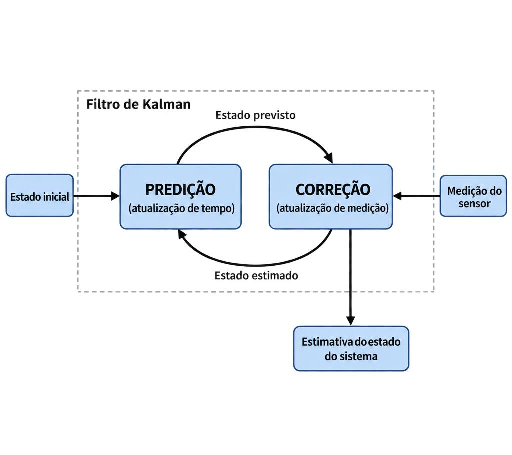
\includegraphics[width=0.8\textwidth]{figuras/fig_filtro_kalman.pdf}
    \caption{Ciclo do Filtro de Kalman: as duas fases, predição (atualização de tempo)
    e correção (atualização de medição), alternam-se indefinidamente, trocando entre si
    o estado previsto e o estado estimado. O filtro é o ciclo, não uma de suas etapas.}
    \legend{Fonte: Elaborada pelo autor.}
    \label{fig:filtro_kalman}
\end{figure}

Para cada etapa temos:

%% Reescrita em 14/11/2026, junto com a figura. A enumeracao anterior tinha tres
%% defeitos: (i) o item 1 dizia que a medicao "nao esta explicitamente rotulada" na
%% figura, o que deixou de ser verdade; (ii) o item 6 listava "Ciclo Recursivo do
%% Filtro de Kalman" como se fosse mais uma etapa, repetindo no texto o erro
%% categorico que a figura antiga cometia -- o ciclo e o conjunto, nao uma etapa; e
%% (iii) a ordem (medicao, correcao, estado estimado, predicao, estado previsto) nao
%% correspondia ao ciclo canonico de duas fases agora desenhado.
\begin{enumerate}
    \item \textbf{Predição (atualização de tempo).} Com base no modelo do sistema --- por exemplo, o modelo de movimento do robô ---, o filtro projeta o estado provável no instante seguinte, propagando também a incerteza associada ao processo. Seu resultado é o \emph{estado previsto}.

    \item \textbf{Medição do sensor.} Chega uma nova observação dos sensores (\ac{IMU}, GPS, \ac{LiDAR}, entre outros), que alimenta a etapa de correção. Ao contrário do estado previsto, ela é informação externa ao modelo.

    \item \textbf{Correção (atualização de medição).} Compara-se a medição com o estado previsto. Da comparação resulta o ganho de Kalman, que pondera quanto o filtro deve confiar na medição atual em relação à previsão. O resultado é o \emph{estado estimado}, melhor estimativa corrente das variáveis de estado: posição, velocidade e demais.

    \item \textbf{Realimentação.} O estado estimado retorna à predição, que projeta o instante seguinte, e o ciclo recomeça. Note-se que o filtro \emph{é} esse ciclo: predição e correção alternam-se indefinidamente, e não existe uma etapa separada à qual caiba o nome de filtro de Kalman.
\end{enumerate}

O Filtro de Kalman é amplamente usado em fusão sensorial para, combinar medições ruidosas e incompletas de múltiplos sensores, obter uma estimativa mais confiável do estado do sistema e também para operar de forma online, ajustando-se em tempo real à medida que novas medições chegam.


Na etapa de predição, o estado atual é estimado com base no estado anterior e no modelo do sistema:

\begin{equation}
\hat{x}_{k|k-1} = F_k\hat{x}_{k-1|k-1} + B_ku_k
\end{equation}

\begin{equation}
P_{k|k-1} = F_kP_{k-1|k-1}F_k^T + Q_k
\end{equation}

Na etapa de atualização, a estimativa é corrigida com base nas medições dos sensores:

\begin{equation}
K_k = P_{k|k-1}H_k^T(H_kP_{k|k-1}H_k^T + R_k)^{-1}
\end{equation}

\begin{equation}
\hat{x}_{k|k} = \hat{x}_{k|k-1} + K_k(z_k - H_k\hat{x}_{k|k-1})
\end{equation}

Para sistemas não-lineares, variantes como o Filtro de Kalman Estendido (\ac{EKF}) e o Filtro de Kalman Unscented (\ac{UKF}) são utilizadas \cite{Costa2018ImplementacaoFusao}.

\subsubsection{Redes Bayesianas}

As redes Bayesianas oferecem um \textit{framework} probabilístico para modelar relações causais entre variáveis, sendo particularmente úteis para fusão sensorial de alto nível \cite{Ramos2012AplicacaoTecnicas}. A probabilidade conjunta de todas as variáveis na rede é dada por:

\begin{equation}
P(X_1, X_2, ..., X_n) = \prod_{i=1}^{n} P(X_i | Pa(X_i))
\end{equation}

Onde $Pa(X_i)$ representa o conjunto de pais do nó $X_i$ no grafo.

Em fusão sensorial, as redes Bayesianas permitem integrar informações de diferentes sensores considerando suas incertezas e relações causais.

\subsubsection{Redes Neurais e Aprendizado Profundo}

Técnicas de aprendizado de máquina, especialmente redes neurais profundas, têm sido cada vez mais aplicadas para fusão sensorial \cite{Wu2022LidarFusionSurvey, Ou2024SensorFusionDRL}. Estas abordagens permitem aprender automaticamente representações e relações complexas entre diferentes modalidades sensoriais.

Arquiteturas comuns incluem Redes Neurais Convolucionais (\ac{CNN}) para processamento de dados espaciais, Redes Neurais Recorrentes (\ac{RNN}) para sequências temporais, e arquiteturas multimodais específicas para combinar diferentes tipos de dados sensoriais.

Uma arquitetura típica de fusão sensorial baseada em aprendizado profundo pode ser representada como:

\begin{equation}
F_{fusão} = f_{fusão}(f_1(X_1), f_2(X_2), ..., f_n(X_n))
\end{equation}

Onde $X_i$ representa os dados do sensor $i$, $f_i$ é a rede neural específica para processar o sensor $i$, e $f_{fusão}$ é a rede de fusão que combina as representações intermediárias.

\subsection{Desafios da Fusão em Ambientes com Interferência Eletromagnética}

A fusão sensorial em subestações elétricas enfrenta desafios específicos devido à
presença de campos eletromagnéticos intensos \cite{He2007EMCSubstation, Yan2024CombinedNav}.
O campo induz ruído e distorção nos próprios sensores eletrônicos, e os magnéticos, os
inerciais e os de comunicação sem fio são os mais suscetíveis. A intensidade e a
distribuição espacial dessa interferência variam ao longo do tempo, de modo que um
conjunto fixo de pesos entre sensores não se sustenta por toda a missão. E a degradação
não é uniforme: cada modalidade é afetada de maneira distinta, o que transfere o problema
da filtragem de um sinal para a estratégia de fusão, que precisa decidir qual leitura
desacreditar e quando. Técnicas de mitigação incluem blindagem eletromagnética, filtragem
digital e algoritmos de detecção e compensação de interferência \cite{Yan2024CombinedNav}.

\subsection{Modelos de Pesos e Bias para Relevância Sensorial}

A ponderação relativa entre sensores determina o resultado da fusão, e precisa refletir a confiabilidade, a relevância e a qualidade momentânea de cada leitura \cite{Neto2021FiltrosRadarLidar, Schneider2018FusaoSensores}.

\subsubsection{Ponderação Baseada em Covariância}

Um método comum para atribuir pesos aos sensores é baseado na matriz de covariância do erro de medição. Sensores com menor incerteza (menor covariância) recebem maior peso. Para o caso de fusão de estimativas escalares de múltiplos sensores, a estimativa ótima é dada por:

\begin{equation}
\hat{x} = \sum_{i=1}^{n} w_i x_i
\end{equation}

Onde os pesos $w_i$ são calculados como:

\begin{equation}
w_i = \frac{\sigma_i^{-2}}{\sum_{j=1}^{n} \sigma_j^{-2}}
\end{equation}

Com $\sigma_i^2$ representando a variância do erro de medição do sensor $i$.

\subsubsection{Ponderação Adaptativa Baseada em Contexto}

Em ambientes dinâmicos como subestações elétricas, a confiabilidade dos sensores pode variar em função do contexto operacional. Modelos adaptativos de ponderação consideram fatores contextuais para ajustar os pesos dos sensores em tempo real \cite{Yan2024CombinedNav}:

\begin{equation}
w_i(t) = f_w(w_i^{base}, c_1(t), c_2(t), ..., c_m(t))
\end{equation}

Onde $w_i(t)$ é o peso do sensor $i$ no instante $t$, $w_i^{base}$ é o peso base do sensor $i$, $c_j(t)$ são fatores contextuais (nível de interferência eletromagnética, iluminação, etc.), e $f_w$ é a função de adaptação dos pesos.

\subsection{Aplicações em Robótica Móvel para Inspeção}

A fusão sensorial heterogênea é particularmente relevante para robôs de inspeção em
subestações elétricas, onde diferentes tipos de sensores são necessários para detectar
diversos tipos de anomalias \cite{Lactec2022, Iberdrola2022}. A detecção de pontos
quentes combina imagem térmica com imagem visual, porque a térmica localiza o excesso de
temperatura e a visual identifica em qual componente ele está. A de descargas parciais
combina sensores acústicos, \ac{UV} e \ac{RF}, nenhum dos quais localiza a descarga
isoladamente. A navegação sob interferência eletromagnética recorre a \ac{LiDAR}, câmeras
e \ac{IMU} em conjunto, pela mesma razão que motiva a ponderação adaptativa da subseção
anterior. E a inspeção visual de corrosão, dano físico e vazamento combina as modalidades
visual, térmica e \ac{UV}, que expõem defeitos de naturezas diferentes na mesma
superfície.

Nenhuma das técnicas de fusão descritas acima é implementada nesta tese. Elas delimitam o que se entende por evento sensorial na Seção~\ref{sec:prop-sensoriamento}, onde a detecção entra no sistema já classificada por modalidade e intensidade, e o objeto de estudo passa a ser a decisão que vem depois dela.
